\documentclass[ngerman]{beamer}


\usepackage[utf8]{inputenc}
\usepackage[T1]{fontenc}
\usepackage{booktabs}
\usepackage{babel}
\usepackage{graphicx}
\usepackage{csquotes}
\usepackage{xcolor}

\author{Dr. Uwe Ziegenhagen}
\title{Grundlagen der Einkommenssteuer in Deutschland}

\begin{document}

\begin{frame}

\maketitle

\end{frame}

\begin{frame}
\frametitle{Disclaimer}

\begin{itemize}
\item Ich bin kein Steuerfachmann
\item Sämtliche Angaben in dieser Präsentation ohne Gewähr
\item Kein Anspruch auf Vollständigkeit
\item Alle Angaben auf Basis besten Wissens und Gewissens
\item Für rechtssichere Auskünfte geht zum Steuerberater oder Finanzamt
\item Thema ist komplex, 10--15\% der Weltsteuerliteratur kommt aus D
\end{itemize}
\end{frame}


\begin{frame}
\frametitle{Inhalt}

\tableofcontents

\end{frame}

\section{Grundlagen}

\begin{frame}
\frametitle{Rechtsgrundlagen}
\framesubtitle{~}

\begin{itemize}
\item Basis für die Erhebung der Einkommenssteuer: EStG (\url{https://www.gesetze-im-internet.de/estg/inhalts_bersicht.html})
\item §1 EStG: \enquote{Natürliche Personen, die im Inland einen Wohnsitz oder ihren gewöhnlichen Aufenthalt haben, sind unbeschränkt einkommensteuerpflichtig.}

\begin{itemize}
	\item Natürliche Personen: Menschen, keine juristischen Personen
	\item Unbeschränkte Steuerpflicht beginnt mit der Geburt bzw. dem Zuzug, endet mit dem Tod bzw. dem Wegzug!
	\item Beschränkt: für Leute, die keinen Wohnsitz haben und sich <183 Tage in Deutschland aufhalten
\end{itemize}
\end{itemize}
\end{frame}


\begin{frame}
\frametitle{Progression}
\framesubtitle{~}

\begin{itemize}
\item Steuerprogression: Ansteigen des Steuersatzes in Abhängigkeit vom zu versteuernden Einkommen oder Vermögen. 
\item $\Rightarrow$ Wer mehr verdient, zahlt proportional mehr Einkommenssteuer!
\item fünf Zonen (Zahlen für 2017) mit jeweils anderen Parametern für die Steuerberechnung
\end{itemize}


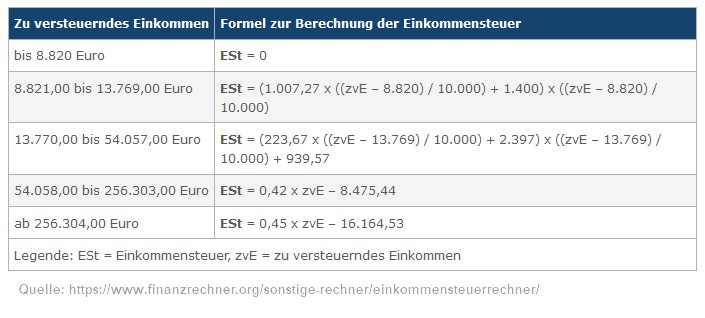
\includegraphics[width=\textwidth]{Bilder/Formeln}

\end{frame}

\begin{frame}
\frametitle{Progression}
\framesubtitle{~}

\textbf{Begriffe}

\begin{description}
\item[Grenzsteuersatz] Mit wieviel \% wird der nächste Euro Einkommen versteuert?
\item[Durchschnittssteuersatz] Wieviel \% des Einkommens gehen für die ESt drauf?
\item[Kalte Progression] Steuermehrbelastung wenn die Variablen eines progressiven Steuertarifes nicht an Inflation angepasst werden.
\end{description}

Beispiel: Jahreseinkommen von 8821 Euro: 8820 Euro sind steuerfrei, nur für den 8821en Euro fallen 0.14 Euro Steuern an.



\end{frame}

\begin{frame}
\frametitle{Einkommen}
\framesubtitle{~}

Sieben Einkommensarten:

\begin{itemize}
\item 
\item 
\item 
\item 
\item 
\item 
\end{itemize}
\end{frame}




\end{document}